
\section{Experimental Results}
\label{sec:experimental_results}

In this section, we present the experimental results of our proposed system. The evaluation of the system is based on the data collected from the experimental setup described in Section~\ref{sec:experimental_setup}. 

The main performance metric used to evaluate the system is the classification accuracy on the test dataset, which is defined as the ratio of the number of correctly classified instances to the total number of instances. We will present the confusion matrix to illustrate the classification results in detail.


\begin{figure}[H]
    \begin{center}
        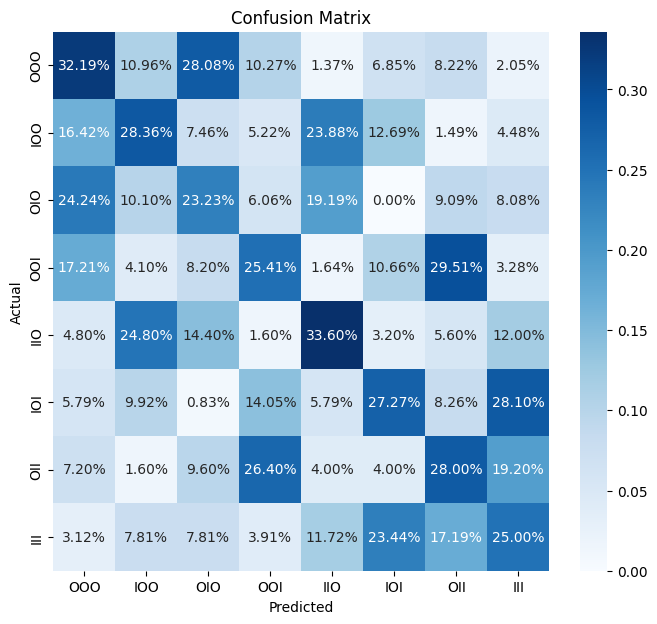
\includegraphics[width=8cm]{Figures/confusion_matrix.png}\vspace{0mm}
        \caption{Confusion matrix illustrating classification results}\vspace{0mm}
        \label{fig:confusion_matrix}
    \end{center}
\end{figure}

The confusion matrix shown in Figure~\ref{fig:confusion_matrix} provides a detailed view of the classification results. The overall accuracy on the test dataset is \textbf{56\%}. As it can be seen from the confusion matrix, the model performs well in classifying the class where all parking spots are empty (OOO) and the class where all parking spots are occupied (III). It is also noteworthy that the model performs well in classifying the class where only one parking spot is occupied (OOI, OIO, and IOO). However, the model confuses the classes where the states of two parking spots are the same and the third one is different. It also struggles to detect the occupancy of the middle parking spot and it confuses IOI with III. We suspected that this could be due to the placement of the Tx and Rx devices, which were placed on the sides of the row of parking spots. Different placement of the Tx and Rx devices were tested to evaluate their impact on the classification performance. However, the results were not significantly different from the ones presented here. While these results are not conclusive and the performance is not high enough for practical applications, they provide a good starting point for further research in this area. When compared to the results of WiParkFind that achieved an accuracy of 76\% when predicting only the number of vehicles in a row of parking spots, our system shows potential for improvement in future iterations.